\documentclass[10pt, twocolumn]{article}

\usepackage[margin=0.75in]{geometry}
\usepackage{amsmath,amsthm,amssymb}
\usepackage{xcolor}
\usepackage{cancel}
\usepackage{graphicx}
\usepackage{changepage}
\usepackage{circuitikz}
\usepackage{pgfplots}
\usepackage{physics}
\usepackage{hyperref}
\usepackage[separate-uncertainty = true,multi-part-units=single]{siunitx}
\usepackage{fontspec}
\usepackage{relsize}
\usepackage{subfig}
\usepackage{minted}
\usepackage{todonotes}
\usepackage{adjustbox}
\usepackage{pdfpages}
\usepackage{multicol, multirow, booktabs}
\usepackage[breakable]{tcolorbox}
\usepackage[inline]{enumitem}
\usepackage{etoolbox}

\theoremstyle{definition}
\newtheorem{problem}{Problem}
\newtheorem{soln}{Solution}

\pgfplotsset{compat=newest}
\usetikzlibrary{lindenmayersystems}
\usetikzlibrary{arrows}
\usetikzlibrary{calc}
\usetikzlibrary{patterns}

\definecolor{incolor}{HTML}{303F9F}
\definecolor{outcolor}{HTML}{D84315}
\definecolor{cellborder}{HTML}{CFCFCF}
\definecolor{cellbackground}{HTML}{F7F7F7}
\newcommand{\ui}{\hat{i}}
\newcommand{\uj}{\hat{j}}
\newcommand{\uk}{\hat{k}}
\newcommand{\ux}{\hat{x}}
\newcommand{\uy}{\hat{y}}
\newcommand{\uz}{\hat{z}}
\newcommand{\primed}[1]{#1^\prime}
\usetikzlibrary{positioning, fit, calc}
\pgfdeclarelayer{background}  
\pgfsetlayers{background,main}
\AtBeginDocument{\RenewCommandCopy\qty\SI}
\definecolor{LightGray}{gray}{0.9}

\makeatletter
\newcommand{\boxspacing}{\kern\kvtcb@left@rule\kern\kvtcb@boxsep}
\makeatother
\newcommand{\prompt}[4]{
    \ttfamily\llap{{\color{#2}[#3]:\hspace{3pt}#4}}\vspace{-\baselineskip}
}

\newcommand{\thevenin}[2]{
  \begin{center}
    \begin{circuitikz} \draw
      (0,0) -- (2,0) to[battery1, l_=$V_{Th}\eq#1$] (2,2) 
      to[resistor, l_=$R_{Th}\eq#2$] (0,2)
      ;
      \draw [o-] (-.07,2.079);
      \draw [o-] (-.07,0.079);
    \end{circuitikz}
  \end{center}
}

\newcommand{\norton}[2]{
  \begin{center}
    \begin{circuitikz} \draw
      (0,0) -- (3,0) to[american current source, l_=$I_{N}\eq#1$] (3,2) -- (0,2) (2,0)
      to[resistor, l=$R_{N}\eq#2$] (2,2)
      ;
      \draw [o-] (-.07,2.079);
      \draw [o-] (-.07,0.079);
    \end{circuitikz}
  \end{center}
}

\newcommand{\highlight}[1]{\colorbox{yellow}{$\displaystyle #1$}}

\newcommand{\ti}[1]{\widetilde{#1}}

\newfontface{\Kaufmann}{Kaufmann}
\DeclareTextFontCommand{\kf}{\Kaufmann}
\newcommand{\scriptr}{\fontsize{12pt}{12pt}\kf{r}}

\newfontface{\KaufmannB}{Kaufmann Bd BT}
\DeclareTextFontCommand{\kfb}{\KaufmannB}
\newcommand{\bscriptr}{\fontsize{12pt}{12pt}\kfb{r}}

\newcommand{\bv}[1]{\mathbf{#1}}

\title{Physics 3200Y: Lab 1}
\author{Jeremy Favro (0805980), Bryan Roberts (0691165) 
 \\\emph{Department of Physics \& Astronomy}\\ Trent University, Peterborough, ON, Canada}
\date{\today}

\begin{document}
\maketitle

\listoftodos
\section{Introduction}
This lab seeks to derive and verify an expression for the potential at every point inside a coaxial cylindrical capacitor.
Herein such a capacitor is constructed and analyzed at a variety of frequencies to determine the validity of the derived equation.
Significant deviation from expected results was observed in extreme regions of the capacitor and is determined to likely be caused
by the invalidation of assumptions made during the derivation of the equation
\section{Theory}
\subsection{Deriving the Potential}
By the integral form of Gauss'
law
$$\oint_{S}\vec{E}\cdot d\vec{a}=\frac{Q_{enc}}{\epsilon_0}$$
in the setup depicted in \ref{fig:coax} a cylindrical Gaussian surface can be constructed, giving an area element
$$d\vec{a}=r\phi d\phi dz\hat{r}.$$
Because the electric field here is unknown it cannot be directly integrated.
Instead an assumption must be made that the electric field solely in the radial direction.
This is reasonable for a capacitor where we can ignore edge effects which would make it invalid.
Using this the $\vec{E}$ term can be extracted from the integral which reduces
to the area of a cylinder. Additionally, as the field is entirely radial
(again ignoring edge effects), the dot product of the vectors reduces
to the product of their only components, both of which are in the radial direction. This yields
$$E=\frac{Q_{enc}}{2\epsilon_0\pi r L}.$$
From this the definition of the potential at some point $\primed{r}$ (neglecting the
vector due, again, to symmetries requiring only a value of radius) relative to an origin $a$ can be applied:
$$V(\primed{r})
  =-\int_{b}^{\primed{r}}E\,dr
  =-\frac{Q_{enc}}{2\epsilon_0\pi L}\int_{b}^{\primed{r}}\frac{dr}{r}
  =\frac{Q_{enc}}{2\epsilon_0\pi L}\ln\left(\frac{\primed{r}}{b}\right).$$
This is inconvenient however as the charge $Q_{enc}$ is unknown.
$V_0=V(a)-V(b)$ is however known as it is the voltage applied between the two cylinders
which can also be determined using the previous equation,
\begin{align*}
           & V_0     =\frac{Q_{enc}}{2\epsilon_0\pi L}\ln\left(\frac{\primed{a}}{b}\right) \\
  \implies & Q_{enc} =\frac{2\epsilon_0\pi L V_0}{\ln\left(a/b\right)}
\end{align*}
which, when substituted back into the equation for potential at arbitrary distance from $b$ gives
$$V(\primed{r})=
  \frac{\ln\left(\primed{r}/b\right)}{\ln\left(a/b\right)}V_0$$
which is entirely in terms of known quantities.
\clearpage
\section{Methods}
\subsection{Coaxial Capacitor}
\todo{image of lab setup}
The first setup involved two coaxial \todo{Maybe talk about alignment}
aluminum cylinders held at known but different potentials (See \ref{fig:coax}). The outer cylinder
with inner radius $r_b\approx\qty{21.25(0.01)}{\centi\meter}$ and the inner (solid) cylinder with radius
$r_a\approx\qty{5.77(0.01)}{\centi\meter}$. The inner cylinder was connected to a variable frequency
function generator set to a root-mean-square (RMS) voltage of $V_{gen}\approx\qty{7.76}{\milli\volt}$.
The outer cylinder was held at ground. Tap water was used as a dielectric and filled the space between the cylinders
at a constant depth.
A Siglent SDS1202X-E oscilloscope was connected to a needle-tip probe. The probe was
used to measure voltage at points on a printed template of $\approx\qty{1}{\centi\meter}$ grid squares.
Measurements were performed under an assumption of perfect radial symmetry
which is a suitable approximation for such a configuration. Measurements
were performed with a fixed input signal RMS voltage of $V_{gen}$ on the intersection of
every neighbouring grid square in a line outward from the inner cylinder. Measurements
were performed at a variety of frequencies to determine if the potential inside the capacitor
has any dependence on frequency.
\todo{Mention code for potential map?}
\subsection{Second Capacitor}
A second capacitor consisting of parallel aluminum plates centered inside the outer cylinder in the original coaxial capacitor
was also studied (see \ref{fig:ppc}). The setup was similar to the coaxial capacitor with the inner element(s)
at a known potential $V_{gen}$ and the outer element at ground. Tap water was again used as a dielectric. The configuration was quadrant-wise symmetric
which allowed measurements to be made for only the upper-left quadrant using the same oscilloscope and need tipped probe as before.
The collected data was then mirrored into the other quadrants using Python.
\newcolumn
\begin{figure}
  \centering
  \begin{minipage}{.5\textwidth}
    \centering
    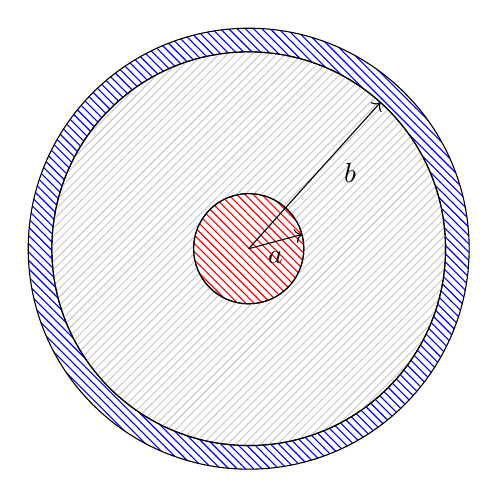
\begin{tikzpicture}
      \def\Rin{0.4}
      \def\Rout{2.5}
      \def\a{0.3}

      % PLATES
      \draw[black,even odd rule, pattern=north west lines, pattern color=red]
      (0,0) circle (0) circle (\Rin+\a); % Inner
      \draw[black,even odd rule, pattern=north west lines, pattern color=blue]
      (0,0) circle (\Rout) circle (\Rout+\a); % Outer
      \draw[even odd rule, pattern=north east lines, pattern color=black!20!white]
      (0,0) circle (\Rin+\a) circle (\Rout); % Water

      \draw[->] (0,0) -- (15:\Rin+\a) node[midway,below] {$a$};
      \draw[->] (0,0) -- (48:\Rout) node[pos=0.65,below right] {$b$};
    \end{tikzpicture}
    \captionof{figure}{Coaxial Capacitor Structure}
    \label{fig:coax}
  \end{minipage}%
  \hspace{.1\textwidth}%
  \begin{minipage}{.5\textwidth}
    \centering
    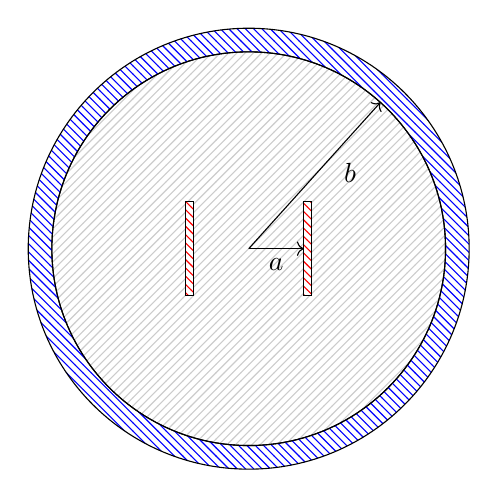
\begin{tikzpicture}
      \def\Rin{0.4}
      \def\Rout{2.5}
      \def\a{0.3}

      % PLATES
      \draw[pattern=north east lines, pattern color=black!20!white]
      (0,0) circle (\Rout); % Water
      \draw[preaction={fill, white}, black, even odd rule, pattern=north west lines, pattern color=red]
      (0,0) ++(-2*\a-0.1, -2*\a) rectangle ++(-0.1, 4*\a)
      (0,0) ++(2*\a+0.1, -2*\a) rectangle ++(+0.1, 4*\a); % Inner
      \draw[black,even odd rule, pattern=north west lines, pattern color=blue]
      (0,0) circle (\Rout) circle (\Rout+\a); % Outer

      \draw[->] (0,0) -- (0:\Rin+\a) node[midway,below] {$a$};
      \draw[->] (0,0) -- (48:\Rout) node[pos=0.65,below right] {$b$};
    \end{tikzpicture}
    \captionof{figure}{Second Capacitor Structure}
    \label{fig:ppc}
  \end{minipage}
\end{figure}

\newpage
\begin{figure}
  \centering
  \begin{minipage}{.5\textwidth}
    \centering
    \includegraphics[width=\linewidth]{Figure_1.png}
    \captionof{figure}{A figure}
    \label{fig:coax-results}
  \end{minipage}%
  \begin{minipage}{.5\textwidth}
    \centering
    \includegraphics[width=\linewidth]{Figure_2.png}
    \captionof{figure}{Another figure}
    \label{fig:coax-residuals}
  \end{minipage}%
\end{figure}
\section{Results}
\subsection{Coaxial Capacitor}
The general curve shape of the derived potential vs. position curve was successfully retrieved for the coaxial capacitor.
There is significant error near the edges of the measured region (see \ref{fig:coax-residuals}).
These regions are where the assumptions made in deriving
the ideal potential equation begin to fall apart as the electric field is no longer radial and begins to curve significantly.
Uncertainty is also present in the position of the probe. No strategies were employed to accurately locate the probe beyond visual inspection.
There does appear to be some dependence on frequency though if it does exist it is fairly subtle and washed out by semi-random error
in the data.
\begin{table}[h]\centering
  \caption{Coaxial Data}
  \begin{tabular}{ccc}
    \toprule
    \textbf{Grid Position} & \textbf{$V_{probe}$ ($\unit{\milli\volt}$)} & \textbf{Frequency ($\unit{\hertz}$)} \\
    \midrule
    I16/J15                & $5150\pm100$                                & 10                                   \\
    I15/H17                & $3930\pm100$                                & -                                    \\
    H17/G18                & $3100\pm100$                                & -                                    \\
    G18/F19                & $2360\pm100$                                & -                                    \\
    F19/E20                & $1770\pm100$                                & -                                    \\
    E20/D21                & $1310\pm100$                                & -                                    \\
    \midrule
    I16/J15                & $5450\pm100$                                & 100                                  \\
    I15/H17                & $4110\pm100$                                & -                                    \\
    H17/G18                & $3220\pm100$                                & -                                    \\
    G18/F19                & $2140\pm100$                                & -                                    \\
    F19/E20                & $1420\pm100$                                & -                                    \\
    E20/D21                & $860\pm100$                                 & -                                    \\
    \midrule
    I16/J15                & $6180\pm100$                                & 1000                                 \\
    I15/H17                & $4560\pm100$                                & -                                    \\
    H17/G18                & $3300\pm100$                                & -                                    \\
    G18/F19                & $2250\pm100$                                & -                                    \\
    F19/E20                & $1430\pm100$                                & -                                    \\
    E20/D21                & $670\pm100$                                 & -
  \end{tabular}
  \label{table:coax-measurements}
\end{table}
\clearpage
\subsection{Second Capacitor}
\begin{figure}
  \centering
  \begin{minipage}{.5\textwidth}
    \centering
    \includegraphics[width=\linewidth]{hplot.png}
    \captionof{figure}{The mapped potentials of the second capacitor.}
    \label{fig:ppc-results}
  \end{minipage}%
  \hspace{.1\textwidth}%
  \begin{minipage}{.5\textwidth}
    \centering
    \includegraphics[width=\linewidth]{hplot-sideon.png}
    \captionof{figure}{Side-on view of \ref{fig:ppc-results}.}
    \label{fig:ppc-results-so}
  \end{minipage}%
  \hspace{.1\textwidth}%
  \begin{minipage}{.5\textwidth}
    \centering
    \includegraphics[width=\linewidth]{hplot-topdown.png}
    \captionof{figure}{Top down view of \ref{fig:ppc-results}. Note the distinct behaviours per ``region''.}
    \label{fig:ppc-results-td}
  \end{minipage}%
\end{figure}
A model was not developed for the second capacitor. It does behave somewhat as expected qualitatively. The capacitor overall exhibits
similar behaviour to that seen in the purely cylindrical case but also behaves similarly to a parallel plate capacitor
near the center. There is again a significant uncertainty in the measurements made due to uncertain probe position, height,
and edge effects.

There are two significant anomalies (which are mirrored in all four quadrants) near the outer edge of the parallel plates.
Both are likely due to the probe being further from the plates than in other measurements as both are in regions where, due to the
mounting system of the probe, it was difficult to center the measuring tip.
\section{Discussion}
\subsection{Sources of Uncertainty}
Systematic uncertainty in the experiment is largely caused by (in order of severity)
\begin{enumerate}
  \item Imprecise probe placement. The exact position of the probe was not precisely determined during each measurement.
        An estimated $\qty{2}{\milli\meter}$ position uncertainty is included in the horizontal error bars in \ref{fig:ppc-results}
        to represent this, though the actual deviation from an ideal measurement is likely significantly more than this in some cases
        and makes determining subtle influences on the equation, such as a potential frequency dependence, difficult.
  \item Imprecise potential measurement. This arises from several factors. Most notably is direct fluctuations
        in the potential displayed by the oscilloscope making it difficult to settle on an exact value.
\end{enumerate}
Error propagation was not performed using any of these uncertainties due to time constraints. Uncertainties were instead estimated
based on the smallest divisions of measurement devices and observed fluctuations.
\subsection {Edge Effect}
While measuring the potentials in lab it was observed that as the probe neared the edges
of the cylindrical capacitor significant fluctuations in the potential displayed by the oscilloscope were observed.
We initially came to the conclusion that this caused
by the probe in some way altering the electric field when placed close enough to an edge.
It was then suggested that the fluctuations observed were due to edge effects. Edge effects are a phenomenon where,
in this specific case, the electric field gains some not insignificant non-radial component. As in our derivation
of the potential we assumed that the electric field was perfectly radial this causes our predicted values to fall away
from the observed values significantly.
\section{Conclusion}
General graph shapes for the modeled coaxial cylinder capacitor were successfully observed in real-world data. Uncertainties in measurements makes
determining additional dependence on other factors such as frequency difficult to determine though data collected across a range of frequencies
does suggest some dependence on frequency not present in the derived equation. Significant deviation from expected results is present in
the regions near the edges, likely due to edge effects invalidating some assumptions made in the derivation of the potential equation.

The second capacitor's potentials were successfully mapped and qualitatively behave as expected.
\section{Appendix}
\subsection{Images}

\begin{figure}
  \centering
  \begin{minipage}{.5\textwidth}
    \centering
    \includegraphics[scale=0.2]{cylcap.png}
    \captionof{figure}{Coaxial cylinder capacitor. Probe visible at left. Mapping template visible beneath the aluminum elements.}
    \label{fig:ppc-results}
  \end{minipage}%
  \hspace{.1\textwidth}%
  \begin{minipage}{.5\textwidth}
    \centering
    \includegraphics[scale=0.2]{ppcap.png}
    \captionof{figure}{Second capacitor. Note that the plates of the inner element were electrically connected during the potential mapping.}
    \label{fig:ppc-results-td}
  \end{minipage}%
\end{figure}
\subsection{Data}
\begin{table}[h]\centering
  \caption{Second Capacitor Data}
  \begin{tabular}{cc}
    \toprule
    \textbf{Grid Position} & \textbf{$V_{probe}$ ($\unit{\milli\volt}$)} \\
    \midrule
    L1                     & $860 \pm10$                                 \\
    L2                     & $1360 \pm10$                                \\
    L3                     & $2020\pm10$                                 \\
    L4                     & $2860\pm10$                                 \\
    L5                     & $3670\pm10$                                 \\
    L6                     & $4580\pm10$                                 \\
    L7                     & $5230\pm10$                                 \\
    L8                     & $5920\pm10$                                 \\
    L9                     & $6300\pm10$                                 \\
    L10                    & $6670\pm10$                                 \\
    L11                    & $6890\pm10$                                 \\
    L12                    & $6980\pm10$                                 \\
    K1                     & $760\pm10$                                  \\
    K2                     & $1220\pm10$                                 \\
    K3                     & $1970\pm10$                                 \\
    K4                     & $2730\pm10$                                 \\
    K5                     & $3660\pm10$                                 \\
    K6                     & $4670\pm10$                                 \\
    K7                     & $5410\pm10$                                 \\
    K8                     & $6010\pm10$                                 \\
    K9                     & $6580\pm10$                                 \\
    K10                    & $6780\pm10$                                 \\
    K11                    & $6950\pm10$                                 \\
    K12                    & $7030\pm10$                                 \\
    J2                     & $1180\pm10$                                 \\
    J3                     & $1800\pm10$                                 \\
    J4                     & $2780\pm10$                                 \\
    J5                     & $3860\pm10$                                 \\
    J6                     & $4810\pm10$                                 \\
    J7                     & $5720\pm10$                                 \\
    J8                     & $6420\pm10$                                 \\
    J9                     & $6730\pm10$                                 \\
    J10                    & $6970\pm10$                                 \\
    J11                    & $7090\pm10$                                 \\
    J12                    & $7130\pm10$                                 \\
    I2                     & $1010\pm10$                                 \\
    I3                     & $1740\pm10$                                 \\
    I4                     & $2450\pm10$                                 \\
    I5                     & $3250\pm10$                                 \\
    I6                     & $4510\pm10$                                 \\
    I7                     & $5340\pm10$                                 \\
    I8                     & $5830\pm10$                                 \\
    I9                     & $6380\pm10$                                 \\
    \dots                  & \dots
  \end{tabular}
  \label{table:cap-measurements}
\end{table}
\clearpage
\subsection{Code}
\inputminted[
  frame=lines,
  framesep=2mm,
  baselinestretch=1.2,
  bgcolor=LightGray,
  fontsize=\footnotesize,
  linenos,
  breaklines
]{python}{plotter.py}
\inputminted[
  frame=lines,
  framesep=2mm,
  baselinestretch=1.2,
  bgcolor=LightGray,
  fontsize=\footnotesize,
  linenos,
  breaklines
]{python}{hplotter.py}
\end{document}